\documentclass[aps,prl,twocolumn,superscriptaddress,nofootinbib]{revtex4-2}
\usepackage[T1]{fontenc}
\usepackage{amsmath,amssymb}
\usepackage{graphicx}
\usepackage{tikz}
\usetikzlibrary{calc}
\usepackage[colorlinks=true,linkcolor=blue,citecolor=blue,urlcolor=blue]{hyperref}

\newcommand{\cH}{\mathcal H}
\newcommand{\su}{\mathfrak{su}}
\newcommand{\Rep}{\operatorname{Rep}}
\newcommand{\qdim}{\operatorname{qdim}}
\newcommand{\VE}{\overline{\chi}_{E_8}}

\begin{document}

\title{Haagerup Conformal Field Theories from the $E_8$ Lattice}

\author{Tzu-Chen Huang}
\affiliation{[Affiliation]}

\date{September 27, 2026}

\begin{abstract}
We construct an explicit rational, unitary chiral algebra $U$ at central
charge $c=8$ whose representation category is the Drinfeld center of
the Haagerup fusion category $\cH_3$. Inside the lattice vertex algebra
of $E_6\oplus A_2$, $U$ is generated by the currents of
$\su(2)_1\oplus\su(2)_{39}$, the stress tensor, and a single weight-two
field made of three vertex operators with relative phase
$(\sqrt{13}+3i\sqrt3)/\sqrt{40}$. Its diagonal modular invariant is a
$c=8$ conformal field theory with the $Z(\cH_3)$ Verlinde lines. The
chiral algebra of the $(E_8)_1$ Wess--Zumino--Witten model is a
holomorphic extension of $U$, and the model carries topological lines
$\cH_3\boxtimes\cH_3^{\rm op}$, as recently proposed. We present the
spectra, exact chiral correlators, the action of the Haagerup lines,
defect Hilbert spaces, and boundary states, and compare with
modular-bootstrap bounds.
\end{abstract}

\maketitle

\textit{Introduction and summary.}---Symmetries of two-dimensional
quantum field theories are implemented by topological line operators.
Dropping the requirement that these lines be invertible leads to
non-invertible symmetries, described by fusion
categories~\cite{FRS,FFRS,BT,CLSWY}. Among these the Haagerup fusion
category $\cH_3$~\cite{Haagerup,AH,Izumi,GS} is the simplest example
that arises from neither finite groups nor affine Lie
algebras~\cite{note-exotic}. It has six simple lines
$1,\alpha,\alpha^2,\rho,\alpha\rho,\alpha^2\rho$ with
\begin{equation}
 \alpha^3=1,\qquad \alpha\rho=\rho\alpha^2,\qquad
 \rho^2=1+\rho+\alpha\rho+\alpha^2\rho,
 \label{eq:H3}
\end{equation}
and $\qdim\rho=d\equiv(3+\sqrt{13})/2$.

Whether $\cH_3$ is the symmetry of a conformal field theory (CFT) has
become a test case for non-invertible symmetries. Anyon chains built
from $\cH_3$ show numerical evidence for a critical point at
$c\approx2$~\cite{Wolf,HLOTT,VLVWOHV,LZR,HJSWZ}. Topological field
theories~\cite{HL,HLS}, a gapless phase with degenerate
vacua~\cite{BSN}, and non-unitary rational candidates~\cite{GKL} with
Haagerup symmetry have also been found. Earlier, building on Izumi's computation of the modular data of the
Drinfeld center $Z(\cH_3)$~\cite{Izumi}, Evans and Gannon~\cite{EG}
found candidate characters of a rational CFT at $c=8$ with these
modular data, related to $(E_8)_1$ and $(E_6)_1\times(A_2)_1$. Recently, Albert,
Honda, Kaidi, and Zheng~\cite{AHKZ} proposed that the $(E_8)_1$
Wess--Zumino--Witten (WZW) model has $\cH_3\times\cH_3^{\rm op}$
symmetry, and obtained it by gauging such a $Z(\cH_3)$ theory, whose
existence they assumed. Gannon and Rayhaun~\cite{GR} showed that its
chiral algebra would be the fixed-point algebra of a hypergroup action
on $(E_6)_1\otimes(A_2)_1$.

In this Letter we construct this theory explicitly. The main results are
as follows. (i)~We give a chiral algebra $U\subset(E_6)_1\otimes(A_2)_1$
at $c=8$, generated by the currents of $\su(2)_1\oplus\su(2)_{39}$, the
stress tensor, and one explicit weight-two field $u$,
Eq.~\eqref{eq:u}. (ii)~$U$ is rational and unitary with
$\Rep(U)\simeq Z(\cH_3)$, and its twelve characters are those
of~\cite{EG}. (iii)~Two full CFTs follow: the diagonal theory of $U$,
whose Verlinde lines form $Z(\cH_3)$, and the $(E_8)_1$ WZW model, whose
lines commuting with $U\otimes\overline U$ form
$\cH_3\boxtimes\cH_3^{\rm op}$. The latter establishes the Haagerup
symmetry of $(E_8)_1$ proposed in~\cite{AHKZ}. (iv)~Because both
theories are rational, their data are exactly computable. We give
spectra, correlators, operator product expansion (OPE) data, twisted
Hilbert spaces, and boundary states.

The existence question reduces to a finite set of exact algebraic
identities in a lattice vertex operator algebra (VOA), together with
further exact checks on explicit fields, all of which we have verified
by computer algebra. The representation theory then follows from
structural arguments. The complete mathematical treatment will
appear in a companion paper~\cite{companion}. Here we concentrate on
the construction and on the physics.

\begin{figure}[t]
\centering
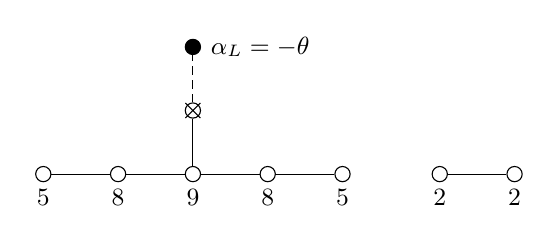
\begin{tikzpicture}[x=0.95cm,y=0.95cm]
 \tikzset{wn/.style={circle,draw,fill=white,inner sep=0pt,minimum size=5.5pt},
          bn/.style={circle,draw,fill=black,inner sep=0pt,minimum size=5.5pt}}
 \foreach \i/\c in {0/5,1/8,2/9,3/8,4/5}{
   \node[wn] (n\i) at (\i,0) {};
   \node[below=2pt,font=\small] at (\i,0) {$\c$};}
 \node[wn] (n5) at (2,0.85) {};
 \draw[line width=0.4pt] ($(n5.center)+(-0.1,-0.1)$)--($(n5.center)+(0.1,0.1)$)
                         ($(n5.center)+(-0.1,0.1)$)--($(n5.center)+(0.1,-0.1)$);
 \node[bn] (nL) at (2,1.7) {};
 \node[right=3pt,font=\small] at (nL) {$\alpha_L=-\theta$};
 \node[wn] (n6) at (5.3,0) {};
 \node[wn] (n7) at (6.3,0) {};
 \node[below=2pt,font=\small] at (5.3,0) {$2$};
 \node[below=2pt,font=\small] at (6.3,0) {$2$};
 \draw (n0)--(n1)--(n2)--(n3)--(n4) (n2)--(n5) (n6)--(n7);
 \draw[densely dashed] (n5)--(nL);
\end{tikzpicture}
\caption{Dynkin diagram of $E_6\oplus A_2$, with the $E_6$ part
extended by its lowest root. The simple roots
$\alpha_0,\dots,\alpha_4$ run left to right along the bottom row of
$E_6$, $\alpha_5$ is the crossed node, and $\alpha_6,\alpha_7$ span
$A_2$. The black node $\alpha_L=-\theta$ generates $\su(2)_1$. The
numbers are the coefficients $c_i$ of the principal $\su(2)$ of
$A_5\oplus A_2$, which generates $\su(2)_{39}$. The three momenta in
$u$ are $a_1=\alpha_6+\alpha_7-\alpha_5$,
$a_2=\alpha_3+\alpha_4-\alpha_5$, and
$a_3=\alpha_0+\alpha_1-\alpha_5$.}
\label{fig:dynkin}
\end{figure}

\textit{The chiral algebra.}---We start from the lattice VOA
$B=V_{E_6\oplus A_2}$, the chiral algebra of the $(E_6)_1\times(A_2)_1$
WZW model, realized by eight chiral bosons $X(z)$ on the $E_6\oplus A_2$
root lattice~\cite{FK,FLM}. Label the simple roots as in
Fig.~\ref{fig:dynkin}, and let $\alpha_L=-\theta$ be the lowest root of
$E_6$. It is orthogonal to the $A_5$ subdiagram
$\alpha_0,\dots,\alpha_4$. The currents
\begin{equation}
 H_{(1)}=\alpha_L\cdot i\partial X,\qquad
 E_{(1)}=e^{i\alpha_L\cdot X}
 \label{eq:su21}
\end{equation}
and their conjugate generate $\su(2)_1$. The principal $\su(2)$
subalgebra of $\su(6)\oplus\su(3)$ has
\begin{equation}
 H_{(39)}=\sum_i c_i\,\alpha_i\cdot i\partial X,\qquad
 E_{(39)}=\sum_i\sqrt{c_i}\,e^{i\alpha_i\cdot X},
 \label{eq:su239}
\end{equation}
with $(c_0,\dots,c_4;c_6,c_7)=(5,8,9,8,5;2,2)$ and $c_5=0$. Its level is
$35+4=39$, the sum of the two embedding indices. The two $\su(2)$
algebras commute. We define
\begin{equation}
 u=e^{ia_1\cdot X}+\zeta\,e^{ia_2\cdot X}+\bar\zeta\,e^{ia_3\cdot X},
 \qquad
 \zeta=\frac{\sqrt{13}+3i\sqrt3}{\sqrt{40}},
 \label{eq:u}
\end{equation}
with the momenta $a_i$ of Fig.~\ref{fig:dynkin}~\cite{note-cocycle}.
All three have $a_i^2=4$, and $a_i\cdot a_j=2$ for $i\ne j$. Note that
$|\zeta|=1$. The field $u$ is a Virasoro primary of weight two. It is
the highest-weight state of spin $(\tfrac12,\tfrac{13}2)$ under
$\su(2)_1\oplus\su(2)_{39}$, with charges $(1,13)$ under
$(H_{(1)},H_{(39)})$. Our chiral algebra is the algebra generated by
these fields under the OPE,
\begin{equation}
 U=\bigl\langle\,\su(2)_1\oplus\su(2)_{39},\ T,\ u\,\bigr\rangle\subset B,
 \label{eq:U}
\end{equation}
where $T$ is the stress tensor of $B$, with $c=8$.

Because $U$ sits inside a lattice VOA, every OPE follows from free-field
Wick contractions, and locality and associativity are automatic. The
nontrivial question is whether $u$ generates a proper subalgebra. It
could instead regenerate the remaining $80$ currents of $B$. We find
that it does not: $U$ is strongly generated by fields of weight at most
four, and
\begin{equation}
 \begin{gathered}
 U_1=\su(2)\oplus\su(2),\\
 \chi_U=q^{-1/3}\bigl(1+6q+120q^2+956q^3+6010q^4+\cdots\bigr).
 \end{gathered}
 \label{eq:charU}
\end{equation}
The stress tensor decomposes into four commuting Virasoro fields,
\begin{equation}
 T=T^{\su(2)_1}+T^{\su(2)_{39}}+T_e+T_f,\quad
 8=1+\tfrac{117}{41}+\tfrac{2400}{1271}+\tfrac{70}{31}.
 \label{eq:Tsplit}
\end{equation}
The $120$ weight-two fields comprise $22$ affine vacuum descendants
($16$ current bilinears and $6$ current derivatives), $T_e$, $T_f$, and
eight multiplets of $\su(2)_1\oplus\su(2)_{39}$ with
dimensions $(1,5)$, $(1,9)^2$, $(1,13)$, $(2,2)$, $(2,6)$, $(2,8)$,
and $(2,14)$. The last multiplet contains $u$. $U$ also contains the
$W$-algebras of the three-state Potts model ($c=\tfrac45$)~\cite{FZ3}
and of the $\mathbb Z_{13}$ parafermions
($c=\tfrac85$)~\cite{ZF}. These echo the numbers $3$ and $13$ in $d$.

We found $u$ by requiring that current descendants of a few
highest-weight fields span the $120$-dimensional weight-two space
predicted by the character, and that their singular OPEs close without
producing the other $80$ currents of $B$. The phase $\zeta$ is the
resulting solution within one ansatz for these fields and one of two
possible current embeddings; we have not established its uniqueness. Closure
in all weights follows from a finite
strong-generation criterion. It reduces to a finite list of OPE
identities, which we verified exactly over
$\mathbb Q(\sqrt{13},\sqrt{-3})$~\cite{companion}. In particular $U\ne B$,
since $\dim B_1=86$. $U$ is stable under the PCT operation of $B$ and
inherits its positive inner product, so it is unitary. Its stress tensor is a positive combination of stress
tensors of rational subalgebras: the two affine algebras and conjugates
of the Potts and parafermion algebras. This implies that $U$ is $C_2$-cofinite and
rational. Combining this with the branching of lattice modules,
fusion-ring and modular-data constraints, the classification of unitary
Haagerup-type categories~\cite{Izumi,GS}, and an analytic argument for
the unitarity of all modules, we find
\begin{equation}
 \Rep(U)\simeq Z(\cH_3)
 \label{eq:RepU}
\end{equation}
as unitary modular tensor categories~\cite{companion}. The characters of $U$ are the
$\gamma=0$ solution of~\cite{EG} [cf.\ Eq.~(12) of~\cite{AHKZ}].

\begin{table}[t]
\caption{The twelve irreducible $U$ modules. Labels follow~\cite{AHKZ},
with those of~\cite{EG} in the second column. Here $h$ is the conformal
weight, $t_M$ the dimension of the lowest-weight space, and
$X=\rho\oplus\alpha\rho\oplus\alpha^2\rho$. The last column is the
restriction $F(M)$ to $\cH_3$, which gives the Haagerup content of the
$E_8$ theory. All sectors are self-conjugate, with twists
$e^{2\pi ih}$.}
\label{tab:sectors}
\begin{ruledtabular}
\begin{tabular}{cccccc}
$M$&\cite{EG}&$h$&$t_M$&$\qdim M$&$F(M)$\\
\hline
$1$&$0$&$0$&$1$&$1$&$1$\\
$\pi_1$&$b$&$1$&$80$&$d^2$&$1\oplus X$\\
$\pi_2$&$a$&$1$&$81$&$2+3d$&$2\cdot1\oplus X$\\
$\sigma_1$&$c_0$&$1$&$81$&$2+3d$&$\alpha\oplus\alpha^2\oplus X$\\
$\sigma_2$&$c_1$&$\tfrac13$&$3$&$2+3d$&$\alpha\oplus\alpha^2\oplus X$\\
$\sigma_3$&$c_2$&$\tfrac23$&$27$&$2+3d$&$\alpha\oplus\alpha^2\oplus X$\\
$\mu_1$&$d_3$&$\tfrac{15}{13}$&$119$&$3d$&$X$\\
$\mu_2$&$d_2$&$\tfrac{11}{13}$&$42$&$3d$&$X$\\
$\mu_3$&$d_4$&$\tfrac{5}{13}$&$5$&$3d$&$X$\\
$\mu_4$&$d_6$&$\tfrac{8}{13}$&$14$&$3d$&$X$\\
$\mu_5$&$d_1$&$\tfrac{6}{13}$&$7$&$3d$&$X$\\
$\mu_6$&$d_5$&$\tfrac{7}{13}$&$13$&$3d$&$X$
\end{tabular}
\end{ruledtabular}
\end{table}

The twelve modules are listed in Table~\ref{tab:sectors}. The modular
$S$ matrix is that of $Z(\cH_3)$~\cite{EG}. The total quantum dimension
is $\mathcal D=3(2+3d)=3+3d^2$, and $\mathcal D^2$ is the global
dimension. As $U$ modules, $(E_6)_1\otimes(A_2)_1$ and, for a suitable
embedding $U\subset V_{E_8}$~\cite{note-H2H3}, $(E_8)_1$ decompose as
\begin{equation}
 (E_6)_1\otimes(A_2)_1=M_1\oplus M_{\pi_1},\qquad
 (E_8)_1=M_1\oplus M_{\pi_1}\oplus2M_{\pi_2}.
 \label{eq:ext}
\end{equation}
For example, the $248$ currents of $E_8$ split as $6+80+81+81$. These
are the chiral counterparts of the gaugings in~\cite{AHKZ}: they
correspond to the commutative algebras $1\oplus\pi_1$ and
$1\oplus\pi_1\oplus2\pi_2$ of $Z(\cH_3)$~\cite{note-H2H3}. The first
exhibits $U$ as the fixed-point algebra anticipated in~\cite{GR}.

\textit{Two full CFTs.}---The diagonal modular invariant
\begin{equation}
 Z_{\rm diag}=\sum_{M}|\chi_M(\tau)|^2
 \label{eq:Zdiag}
\end{equation}
defines a unitary CFT with $c_L=c_R=8$ and twelve
$U\otimes\overline U$ primaries. We call it the $Z(\cH_3)$ theory. Its
topological lines commuting with $U\otimes\overline U$ are the twelve
Verlinde lines~\cite{Verlinde,PZ}. Their fusion rules are those of
$Z(\cH_3)$, and $L_a$ acts on sector $M_i\otimes\overline{M_i}$ by
$S_{ai}/S_{1i}$.

The second full CFT is the $(E_8)_1$ WZW model,
$Z_{E_8}=|\chi_{E_8}|^2$ with $\chi_{E_8}=E_4/\eta^8$. By
Eq.~\eqref{eq:ext}, it is the extension of $U\otimes\overline U$ by the
Lagrangian algebra $A=1\oplus\pi_1\oplus2\pi_2$ in each chirality. Its
topological lines commuting with $U\otimes\overline U$ therefore form
$\Rep(U)_A\boxtimes\Rep(U)_A^{\rm op}$, where $\Rep(U)_A$ is the
category of all (not necessarily local) $A$-modules~\cite{FRS,DMNO}. For
this $A$, $\Rep(U)_A\simeq\cH_3$. The $(E_8)_1$ WZW model therefore has
$\cH_3\boxtimes\cH_3^{\rm op}$ symmetry, as proposed
in~\cite{AHKZ}. These lines commute with $U$ but not with the full
$E_8$ current algebra. Gauging the diagonal $\cH_3$ returns the
$Z(\cH_3)$ theory~\cite{AHKZ}.

Below we mostly use the first factor $\cH_3\boxtimes1$, which acts on
the left movers only. The untwisted Hilbert space is
$(M_1\oplus M_{\pi_1}\oplus\mathbb C^2\otimes M_{\pi_2})\otimes
\overline{V}_{E_8}$. In a suitable basis the lines act as
\begin{equation}
 \widehat\alpha=\bigl(1,\,1,\,\mathrm{diag}(\omega,\omega^2)\bigr),\qquad
 \widehat\rho=\bigl(d,\,-d^{-1},\,\sigma_x\bigr),
 \label{eq:action}
\end{equation}
with $\omega=e^{2\pi i/3}$. They satisfy Eq.~\eqref{eq:H3}. In
particular, the $248$ currents split into $6$ that are invariant
($\widehat\rho=d=\langle\rho\rangle$), $80$ with $\widehat\alpha=1$ and
$\widehat\rho=-d^{-1}$, and $2\times81$ with $\widehat\alpha=\omega^{\pm1}$
that $\widehat\rho$ exchanges. The $\alpha$-invariant subalgebra
$U\oplus M_{\pi_1}$ has the character of $(E_6)_1\otimes(A_2)_1$,
consistent with identifying $\alpha$ with the $\mathbb Z_3$ automorphism
of $E_8$ of class 3B~\cite{AHKZ}. On the $\mathbb Z_3$-neutral states
$\widehat\rho$ takes the two values $(3\pm\sqrt{13})/2$, just as in the
lattice model at $c\approx2$~\cite{HLOTT}; see Fig.~\ref{fig:spectrum}(b).
The twined partition functions are
\begin{equation}
 Z^{[\alpha]}=(\chi_1+\chi_{\pi_1}-\chi_{\pi_2})\VE,\quad
 Z^{[\rho]}=(d\chi_1-d^{-1}\chi_{\pi_1})\VE.
 \label{eq:twined}
\end{equation}
The defect Hilbert spaces follow from the restriction $F$ in
Table~\ref{tab:sectors}:
\begin{equation}
 Z_\alpha=\Bigl(\sum_{i=1}^3\chi_{\sigma_i}\Bigr)\VE,\quad
 Z_\rho=\Bigl(\sum_{M\ne1}\chi_M\Bigr)\VE.
 \label{eq:twisted}
\end{equation}
These are chiral versions of Eqs.~(15)--(16) of~\cite{AHKZ}. Spins in the
$\alpha$-twisted sector lie in $\tfrac13\mathbb Z$, as expected for a
non-anomalous $\mathbb Z_3$. The $\rho$-twisted sector contains
the additional spins $6j^2/13\bmod1$, i.e.\
$\{\tfrac2{13},\tfrac5{13},\tfrac6{13},\tfrac7{13},\tfrac8{13},\tfrac{11}{13}\}$.
In both sectors the lightest defect operator has
$(h,\bar h)=(\tfrac13,0)$, with multiplicity three.

\begin{figure*}[t]
\centering
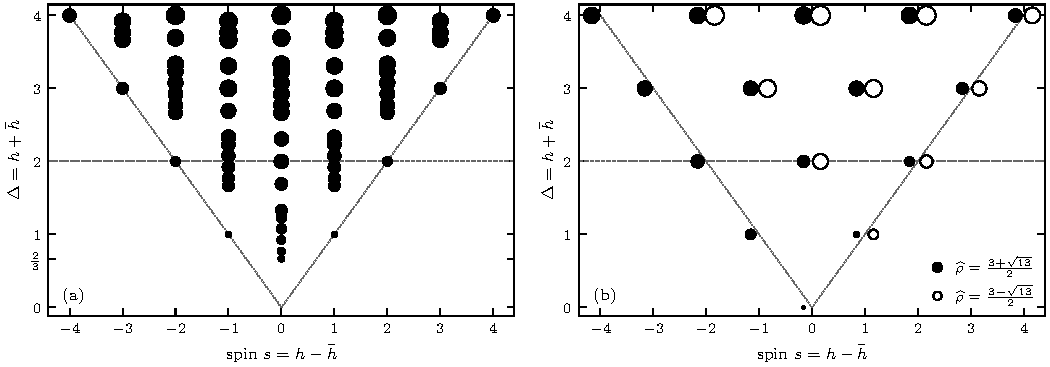
\includegraphics[width=\textwidth]{figures/spectrum.pdf}
\caption{Exact Virasoro-primary spectra; marker area grows with the
logarithm of the multiplicity. (a)~The diagonal $Z(\cH_3)$ theory for
$0<\Delta\le4$. The seven relevant scalar levels are listed in
Eq.~\eqref{eq:relevant}. (b)~The $(E_8)_1$ WZW model, showing the
$\mathbb Z_3$-neutral states of the first-factor $\cH_3$ action with
$\Delta\le4$, including the identity. Filled markers:
$\widehat\rho=(3+\sqrt{13})/2$, i.e.\ $M_1\otimes\overline V_{E_8}$.
Hollow markers: $\widehat\rho=(3-\sqrt{13})/2$, i.e.\
$M_{\pi_1}\otimes\overline V_{E_8}$; where both occur, they are offset
horizontally. Compare Fig.~6
of~\cite{HLOTT}. Dashed lines: $\Delta=2$. Dotted lines: $\Delta=|s|$.}
\label{fig:spectrum}
\end{figure*}

\textit{Spectrum.}---Because all conformal weights are known, the
spectrum follows from the characters. Removing Virasoro descendants is
straightforward at $c=8>1$, where Verma modules of positive weight are
irreducible. Table~\ref{tab:compare} and Fig.~\ref{fig:spectrum}
summarize the two theories. The diagonal theory has seven relevant
scalar levels,
\begin{equation}
 \begin{array}{c|ccccccc}
 \Delta&\tfrac23&\tfrac{10}{13}&\tfrac{12}{13}&\tfrac{14}{13}&
 \tfrac{16}{13}&\tfrac43&\tfrac{22}{13}\\\hline
 \text{mult.}&9&25&49&169&196&729&1764
 \end{array}
 \label{eq:relevant}
\end{equation}
coming from $\sigma_2,\mu_3,\mu_5,\mu_6,\mu_4,\sigma_3,\mu_2$. Each
multiplicity is $t_M^2$. The lightest scalar, at $\Delta=\tfrac23$,
transforms as $(\mathbf1,\mathbf3)\otimes\overline{(\mathbf1,\mathbf3)}$
under the currents. Including spin, there are $10623$ relevant
Virasoro primaries. At $\Delta=2$ there are
$80^2+81^2+81^2+6^2=19558$ scalar primaries. The $E_8$ theory has
scalar gap $2$ and no relevant scalar.

\begin{table}[b]
\caption{The two full CFTs, with $c_L=c_R=8$. Degeneracies count
Virasoro primaries. ``Symmetric'' means invariant under all Verlinde
lines (diagonal theory) or under the first-factor $\cH_3$ ($E_8$
theory).}
\label{tab:compare}
\begin{ruledtabular}
\begin{tabular}{lcc}
&$Z(\cH_3)$ theory&$(E_8)_1$ WZW\\
\hline
Currents per chirality&$6$&$248$\\
Lightest primary $\Delta$&$\tfrac23$&$1$\\
Lightest scalar $\Delta$&$\tfrac23$&$2$\\
Relevant scalars&$2941$&$0$\\
Scalars at $\Delta=2$&$19558$&$61504$\\
Symmetric scalar gap (mult.)&$2\ (36)$&$2\ (1488)$\\
Lines commuting with $U\otimes\overline U$&$Z(\cH_3)$&$\cH_3\boxtimes\cH_3^{\rm op}$
\end{tabular}
\end{ruledtabular}
\end{table}

Neither theory has a symmetric relevant deformation. The $E_8$ theory
has no relevant scalar at all. In the diagonal theory, a sector fixed by
all Verlinde lines has
$S_{ai}/S_{1i}=\qdim L_a$ for every $a$, which forces $i=1$ because $S$
is invertible. The symmetric operators are therefore those of
$U\otimes\overline U$, and the lightest symmetric scalars are the $36$
current bilinears $J^a\bar J^b$ at $\Delta=2$. All $2941$ relevant
scalars are charged, so the $Z(\cH_3)$ symmetry alone keeps the diagonal
theory critical without tuning. In the $E_8$ theory the
$\cH_3$-invariant subspace is $U\otimes\overline V_{E_8}$, with lightest
scalars $J^a_U\bar J^B_{E_8}$.

\textit{Correlators and OPE data.}---The lattice realization gives
explicit interacting correlators. Let $\hat u=u/\sqrt3$ be the unit
normalized field and $\hat u^\dagger$ its conjugate. Its four-point
functions are rational:
\begin{align}
 \langle\hat u^\dagger(\infty)\hat u(1)\hat u^\dagger(x)\hat u(0)\rangle
 &=\frac{3-4x+4x^2}{3x^4(1-x)^4},\label{eq:G0}\\
 \langle\hat u^\dagger(\infty)\hat u^\dagger(1)\hat u(x)\hat u(0)\rangle
 &=\frac{x^2(4-4x+3x^2)}{3(1-x)^4}.\label{eq:Gp}
\end{align}
In the neutral channel, write
$x^4G=A_0+\sum_{n\ge1}A_nx^n{}_2F_1(n,n;2n;x)$.
Then
$(A_0,\dots,A_4)=(1,\tfrac83,\tfrac{14}3,\tfrac{58}9,\tfrac{107}{15})$.
Here $A_1=\tfrac12+\tfrac{13}6$ is the exchange of the two Cartan
currents. The stress tensor contributes $2h^2/c=1$ to $A_2$, and the
remaining $\tfrac{11}3$ is the sum of squared OPE coefficients of
$\hat u\times\hat u^\dagger$ into weight-two Virasoro primaries. In the
equal-charge channel, the OPE $\hat u\times\hat u$ starts at $x^2$ with a
single weight-six primary of squared coefficient $\tfrac43$.

Beyond these, we computed every three-point coefficient among the $113$
weight-two Virasoro primaries of $U$. Of these $18365$ are nonzero; all
are exact, with squared magnitudes in $\mathbb Q(\sqrt{13})$. We also
computed the four-point functions of the spin-three generators of the
embedded Potts and parafermion algebras. Together with spectra through
$\Delta=24$ and the defect and boundary data below, these are provided
as ancillary files.

\textit{Boundaries.}---The diagonal theory has twelve Cardy
states~\cite{Cardy}, with $g$-values
$g_a=\qdim M_a/\sqrt{\mathcal D}$. The $E_8$ theory has six elementary
$U$-preserving boundaries, labeled by $x\in\cH_3$. Their annulus
partition functions are
$Z_{xy}=\sum_{z,M}N_{x^*y}^{\ z}\,n_{zM}\,\chi_M$, where
$n_{zM}=\dim\mathrm{Hom}(F(M),z)$. Their $g$-values are $1$ for $x$
invertible and $d$ for $x=\alpha^k\rho$. The invertible boundaries are
the ordinary $E_8$ boundary and its $\mathbb Z_3$ images. Each
$\rho$-type boundary supports nine relevant boundary operators of
weight $\tfrac13$.

\textit{Bootstrap.}---In the ordinary modular bootstrap~\cite{CLY}, the
$E_8$ theory sits at the known kink $(c,\Delta_{\rm scalar})=(8,2)$,
and the diagonal theory at $(8,\tfrac23)$. For the Haagerup-symmetric bootstrap
of~\cite{AHKZ}, based on the methods of~\cite{LS19,LS23}, the relevant sector functions are
$\chi_M\VE$~\cite{note-bootstrap}. They give an $\cH_3$-invariant
scalar gap $\Delta=2$, and a scalar gap $\Delta=2$ in the
$\mathbb Z_3$-charged tube sectors $\pi_2\cup\sigma_1$. Both points lie
inside the allowed regions of Figs.~2 and~3 of~\cite{AHKZ}, below the
numerical bounds at $c=8$. The bounds are therefore not saturated by
these theories.

\textit{Discussion and outlook.}---We have given an explicit, rational,
and unitary CFT whose topological lines realize the Haagerup category
$\cH_3$ and its center. The construction is elementary: eight free
bosons, the currents of Eqs.~\eqref{eq:su21}--\eqref{eq:su239}, and
the field $u$ of Eq.~\eqref{eq:u}.

\emph{Conformal manifolds with Haagerup symmetry.} The lines
of~\eqref{eq:action} commute with the currents of $U$ and with all
antiholomorphic $E_8$ currents. Deformations by $J^a_U\bar J^b$, with
$J^a_U$ the two Cartan currents of $U$ and $\bar J^b$ the eight Cartan
currents of $\overline{E}_8$, are exactly marginal~\cite{FR}. They span
a family of Narain CFTs locally isomorphic to $O(2,8)/O(2)\times O(8)$,
before global identifications.
Because the perturbing operator passes through every first-factor line,
standard arguments~\cite{CLSWY} suggest that the $\cH_3$ symmetry
survives on this sixteen-dimensional family, most of which is
irrational. The second factor $\cH_3^{\rm op}$ is generically broken.
Likewise, the $Z(\cH_3)$ Verlinde lines of the diagonal theory should
survive its four $J_U\bar J_U$ deformations. Establishing this would
give continuous families of CFTs with a unique vacuum and Haagerup (or
$Z(\cH_3)$) symmetry, in the spirit of the non-invertible symmetries found along
the $c=1$ moduli space~\cite{TW}.

\emph{Bulk OPE and crossing.} The OPE of the nonvacuum sectors of the
diagonal theory is not yet computed, beginning with the nine
$\Delta=\tfrac23$ scalars. Lattice intertwiners give explicit chiral
blocks. For instance the lightest module has blocks
$x^{-2/3}(1-x)^{-\beta_i\cdot\beta_j}$, where $\beta_i$ are the $A_2$
weights. Sewing these into single-valued correlators would provide a
fully solvable benchmark for bootstraps with non-invertible
symmetry~\cite{LS23}.

\emph{Relation to $c\approx2$.} Our theories are not the continuum
limit of the $\cH_3$ anyon chains~\cite{HLOTT,VLVWOHV}.
In~\cite{AHKZ} it was proposed that asymmetric quotients related to
$(A_2)_1$ and $(E_6)_1$ yield Haagerup-symmetric theories at $c=2$ and
$6$, where the bootstrap bounds have kinks. Our explicit chiral algebra
may help to test this.

\emph{Other exotic categories.} Gannon, Schopieray, and Yadav have now
constructed Haagerup--Izumi categories for every odd cyclic group and
proven the Evans--Gannon form of their centers~\cite{GSY}. A natural
next step is to realize these centers by chiral subalgebras of lattice
VOAs. Our method provides a template: guess generators from the
predicted character, then certify closure with a finite
strong-generation criterion. It would also be interesting to find
Haagerup-symmetric lattice models whose continuum limit is the
$c=8$ theory, and to study the relevant boundary perturbations above.

Exact characters, spectra, OPE tensors, and defect and boundary data
accompany this preprint.

\begin{acknowledgments}
[To be added.]
\end{acknowledgments}

\begin{thebibliography}{99}

\bibitem{FRS}
J.~Fuchs, I.~Runkel, and C.~Schweigert,
TFT construction of RCFT correlators I: Partition functions,
\href{https://doi.org/10.1016/S0550-3213(02)00744-7}{Nucl.\ Phys.\ \textbf{B646}, 353 (2002)}.

\bibitem{FFRS}
J.~Fr\"ohlich, J.~Fuchs, I.~Runkel, and C.~Schweigert,
Duality and defects in rational conformal field theory,
Nucl.\ Phys.\ \textbf{B763}, 354 (2007).

\bibitem{BT}
L.~Bhardwaj and Y.~Tachikawa,
On finite symmetries and their gauging in two dimensions,
J.\ High Energy Phys.\ 03 (2018) 189.

\bibitem{CLSWY}
C.-M.~Chang, Y.-H.~Lin, S.-H.~Shao, Y.~Wang, and X.~Yin,
Topological defect lines and renormalization group flows in two
dimensions,
J.\ High Energy Phys.\ 01 (2019) 026.

\bibitem{Haagerup}
U.~Haagerup,
Principal graphs of subfactors in the index range
$4<[M{:}N]<3+\sqrt2$,
in \textit{Subfactors} (World Scientific, River Edge, NJ, 1994),
pp.~1--38.

\bibitem{AH}
M.~Asaeda and U.~Haagerup,
Exotic subfactors of finite depth with Jones indices $(5+\sqrt{13})/2$
and $(5+\sqrt{17})/2$,
Commun.\ Math.\ Phys.\ \textbf{202}, 1 (1999).

\bibitem{Izumi}
M.~Izumi,
The structure of sectors associated with Longo--Rehren inclusions II:
Examples,
Rev.\ Math.\ Phys.\ \textbf{13}, 603 (2001).

\bibitem{GS}
P.~Grossman and N.~Snyder,
Quantum subgroups of the Haagerup fusion categories,
Commun.\ Math.\ Phys.\ \textbf{311}, 617 (2012).

\bibitem{note-exotic}
Most known fusion categories arise from finite groups or quantum
groups by standard constructions; $\cH_3$ does not~\cite{HLOTT}.

\bibitem{Wolf}
R.~Wolf,
Microscopic models for fusion categories,
Ph.D.\ thesis, Leibniz Universit\"at Hannover, 2020,
\href{https://arxiv.org/abs/2101.04154}{arXiv:2101.04154}.

\bibitem{HLOTT}
T.-C.~Huang, Y.-H.~Lin, K.~Ohmori, Y.~Tachikawa, and M.~Tezuka,
Numerical Evidence for a Haagerup Conformal Field Theory,
Phys.\ Rev.\ Lett.\ \textbf{128}, 231603 (2022).

\bibitem{VLVWOHV}
R.~Vanhove, L.~Lootens, M.~Van Damme, R.~Wolf, T.~J.~Osborne,
J.~Haegeman, and F.~Verstraete,
Critical Lattice Model for a Haagerup Conformal Field Theory,
Phys.\ Rev.\ Lett.\ \textbf{128}, 231602 (2022).

\bibitem{LZR}
Y.~Liu, Y.~Zou, and S.~Ryu,
Operator fusion from wavefunction overlaps: Universal finite-size
corrections and application to Haagerup model,
Phys.\ Rev.\ B \textbf{107}, 155124 (2023).

\bibitem{HJSWZ}
L.-Y.~Hung, K.~Ji, C.~Shen, Y.~Wan, and Y.~Zhao,
A 2D-CFT factory: Critical lattice models from competing anyon
condensation processes in SymTO/SymTFT,
\href{https://arxiv.org/abs/2506.05324}{arXiv:2506.05324}.

\bibitem{HL}
T.-C.~Huang and Y.-H.~Lin,
Topological field theory with Haagerup symmetry,
J.\ Math.\ Phys.\ \textbf{63}, 042306 (2022).

\bibitem{HLS}
T.-C.~Huang, Y.-H.~Lin, and S.~Seifnashri,
Construction of two-dimensional topological field theories with
non-invertible symmetries,
J.\ High Energy Phys.\ 12 (2021) 028.

\bibitem{BSN}
L.~E.~Bottini and S.~Schafer-Nameki,
A Gapless Phase with Haagerup Symmetry,
Phys.\ Rev.\ Lett.\ \textbf{134}, 191602 (2025).

\bibitem{GKL}
D.~Gang, D.~Kim, and S.~Lee,
A non-unitary bulk-boundary correspondence: Non-unitary Haagerup RCFTs
from S-fold SCFTs,
SciPost Phys.\ \textbf{17}, 064 (2024).

\bibitem{EG}
D.~E.~Evans and T.~Gannon,
The exoticness and realisability of twisted Haagerup--Izumi modular
data,
Commun.\ Math.\ Phys.\ \textbf{307}, 463 (2011).

\bibitem{AHKZ}
J.~Albert, Y.~Honda, J.~Kaidi, and Y.~Zheng,
Haagerup Symmetry in $(E_8)_1$?,
Phys.\ Rev.\ Lett.\ \textbf{136}, 091603 (2026).

\bibitem{GR}
T.~Gannon and B.~C.~Rayhaun,
Hypergroup symmetry in relative quantum field theories and chiral
algebras,
\href{https://arxiv.org/abs/2606.05279}{arXiv:2606.05279}.

\bibitem{companion}
T.-C.~Huang, A central-charge-eight conformal field theory with
Haagerup symmetry: construction, spectrum and observables (to be
published).

\bibitem{FK}
I.~B.~Frenkel and V.~G.~Kac,
Basic representations of affine Lie algebras and dual resonance models,
Invent.\ Math.\ \textbf{62}, 23 (1980).

\bibitem{FLM}
I.~Frenkel, J.~Lepowsky, and A.~Meurman,
\textit{Vertex Operator Algebras and the Monster}
(Academic Press, Boston, 1988).

\bibitem{note-cocycle}
Vertex operators $e^{ia\cdot X}$ include the cocycle
$\epsilon(a,b)=(-1)^{\sum_ia_ib_i+\sum_{i>j}a_ib_jG_{ij}}$, with $a,b$
in simple-root coordinates and $G$ the Cartan matrix; the lowering
currents are then $-e^{-i\alpha_L\cdot X}$ and
$-\sum_i\sqrt{c_i}\,e^{-i\alpha_i\cdot X}$. The value of $\zeta$ refers
to these conventions.

\bibitem{FZ3}
V.~A.~Fateev and A.~B.~Zamolodchikov,
Conformal quantum field theory models in two dimensions having $Z_3$
symmetry,
Nucl.\ Phys.\ \textbf{B280}, 644 (1987).

\bibitem{ZF}
A.~B.~Zamolodchikov and V.~A.~Fateev,
Nonlocal (parafermion) currents in two-dimensional conformal quantum
field theory and self-dual critical points in $Z_N$-symmetric
statistical systems,
Sov.\ Phys.\ JETP \textbf{62}, 215 (1985).

\bibitem{note-H2H3}
For the extension $U\subset V_{E_8}$ inherited from the lattice, our
argument identifies its category of modules only up to $\cH_3$ and its
Morita-equivalent partner $\cH_2$~\cite{GS,AHKZ}; since
$\chi_{\pi_2}=\chi_{\sigma_1}$, characters cannot tell them apart. An
extension realizing Eq.~\eqref{eq:ext} with $\Rep(U)_A\simeq\cH_3$
exists~\cite{companion} and is used throughout.

\bibitem{Verlinde}
E.~Verlinde,
Fusion rules and modular transformations in 2D conformal field theory,
Nucl.\ Phys.\ \textbf{B300}, 360 (1988).

\bibitem{PZ}
V.~B.~Petkova and J.-B.~Zuber,
Generalised twisted partition functions,
Phys.\ Lett.\ B \textbf{504}, 157 (2001).

\bibitem{DMNO}
A.~Davydov, M.~M\"uger, D.~Nikshych, and V.~Ostrik,
The Witt group of non-degenerate braided fusion categories,
J.\ Reine Angew.\ Math.\ \textbf{677}, 135 (2013).

\bibitem{Cardy}
J.~L.~Cardy,
Boundary conditions, fusion rules and the Verlinde formula,
Nucl.\ Phys.\ \textbf{B324}, 581 (1989).

\bibitem{CLY}
S.~Collier, Y.-H.~Lin, and X.~Yin,
Modular bootstrap revisited,
J.\ High Energy Phys.\ 09 (2018) 061.

\bibitem{LS19}
Y.-H.~Lin and S.-H.~Shao,
$\mathbb Z_N$ symmetries, anomalies, and the modular bootstrap,
Phys.\ Rev.\ D \textbf{100}, 025013 (2019).

\bibitem{LS23}
Y.-H.~Lin and S.-H.~Shao,
Bootstrapping noninvertible symmetries,
Phys.\ Rev.\ D \textbf{107}, 125025 (2023).

\bibitem{note-bootstrap}
The sector functions are $Z_M=\chi_M\VE$, not the diagonal $|\chi_M|^2$.
The tube-algebra multiplicity spaces exclude the finite factors
$\mathrm{Hom}(F(M),x)$. In particular the untwisted $\pi_2$ block
appears twice in the Hilbert space but only once in the bootstrap
vector.

\bibitem{FR}
S.~F\"orste and D.~Roggenkamp,
Current-current deformations of conformal field theories, and WZW
models,
J.\ High Energy Phys.\ 05 (2003) 071.

\bibitem{TW}
R.~Thorngren and Y.~Wang,
Fusion category symmetry II: Categoriosities at $c=1$ and beyond,
\href{https://arxiv.org/abs/2106.12577}{arXiv:2106.12577}.

\bibitem{GSY}
T.~Gannon, A.~Schopieray, and H.~Yadav,
On Haagerup--Izumi fusion categories,
\href{https://arxiv.org/abs/2609.25185}{arXiv:2609.25185}.

\end{thebibliography}

\end{document}
